% 5-minute talk by Jianxiang He: the whole study, Q1–Q4. Script: script_jianxiang.md
\documentclass[aspectratio=169,11pt]{beamer}
% Shared preamble and frames for the three 5-minute talks.
% Each talk sets \presenter{...} before % Shared preamble and frames for the three 5-minute talks.
% Each talk sets \presenter{...} before % Shared preamble and frames for the three 5-minute talks.
% Each talk sets \presenter{...} before \input{common}.
\usepackage{amsmath,amssymb}
\usepackage{booktabs}
\usepackage{xcolor}
\usetheme{MBZUAI}
\graphicspath{{assets/}{../figs/}}
\setbeamertemplate{navigation symbols}{}

\newcommand{\lam}{\lambda}
\newcommand{\strong}[1]{\textcolor{mbzuai-navy}{\textbf{#1}}}
\newcommand{\good}[1]{\textcolor{green!45!black}{\textbf{#1}}}
\newcommand{\bad}[1]{\textcolor{red!65!black}{\textbf{#1}}}

% ── Team and roles: edit here, all three decks update ─────────────────────
\newcommand{\roleJH}{Problem and setup; score cache and data pipeline; Q1 analysis; overall study (Q1--Q4)}
\newcommand{\roleLJ}{Continual learning experiments and analysis (Q2--Q3)}
\newcommand{\roleMA}{Downstream question-answering evaluation (Q4)}

\title[Fusion Weight for Keyframe Search]{Should the Fusion Weight Change with the Question?}
\institute[MBZUAI]{CV805 Course Project \\ Mohamed bin Zayed University of Artificial Intelligence}
\date{\today}
\titlelogos{assets/logo_dark.pdf}
\footleft{Should the Fusion Weight Change with the Question?}
\footright{\insertframenumber{} / \inserttotalframenumber}

% Team slide; #1 = JH, LJ or MA, the presenter's row is highlighted.
\usepackage{etoolbox}
\newcommand{\teamrow}[4]{% #1 key, #2 presenter key, #3 name, #4 role
  \ifstrequal{#1}{#2}%
    {\textbf{\textcolor{mbzuai-navy}{#3}} & \textbf{\textcolor{mbzuai-navy}{#4}} & \textcolor{mbzuai-dark-sand}{\textbf{this talk}}}%
    {\textcolor{mbzuai-subtle}{#3} & \textcolor{mbzuai-subtle}{#4} & }}
\newcommand{\teamframe}[1]{%
\begin{frame}{Team and my part}
  \centering
  \renewcommand{\arraystretch}{1.6}
  \begin{tabular}{p{0.27\textwidth}p{0.52\textwidth}p{0.11\textwidth}}
    \toprule
    Member & Main contribution & \\
    \midrule
    \teamrow{JH}{#1}{Jianxiang He}{\roleJH} \\
    \teamrow{LJ}{#1}{Longtao Jiang}{\roleLJ} \\
    \teamrow{MA}{#1}{Makhmud Assentay}{\roleMA} \\
    \bottomrule
  \end{tabular}
\end{frame}}

% Context frame used by every talk: VSI, the weight, and the example.
\newcommand{\contextframe}{%
\begin{frame}{Background: two clues, one weight}
  \begin{columns}[c,onlytextwidth]
    \begin{column}{0.47\textwidth}
      \small
      A VLM can only look at \strong{about 8 frames} of a long video, so we must pick them well.\\[2mm]
      VSI scores every second with two clues:
      \begin{itemize}
        \item \strong{Visual}: do the question's objects appear?
        \item \strong{Subtitle}: does the subtitle match the question?
      \end{itemize}
      \[ S(t) = (1-\lam)\,\text{visual}(t) + \lam\,\text{subtitle}(t) \]
      and keeps the top 8 seconds. VSI uses \strong{$\lam=0.3$ for every question}.
    \end{column}
    \begin{column}{0.5\textwidth}
      \centering
      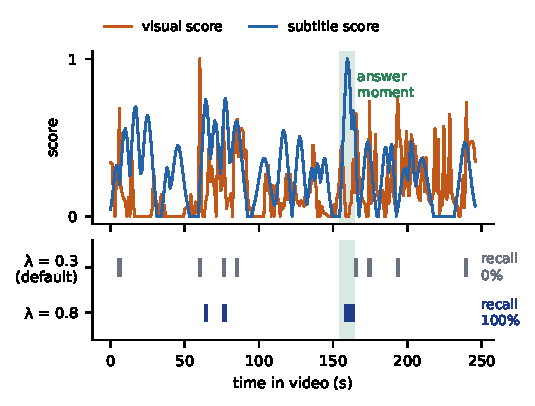
\includegraphics[width=\linewidth]{f01_teaser.pdf}\\
      {\scriptsize Real example: $\lam=0.3$ \bad{misses} the answer moment (green), $\lam=0.8$ \good{hits} it.}
    \end{column}
  \end{columns}
\end{frame}}

\newcommand{\titleframe}{%
{\setbeamertemplate{footline}{}\setbeamertemplate{frametitle}{}
\begin{frame}[t]\titlepage\end{frame}}}

\newcommand{\thankframe}{%
{\setbeamertemplate{footline}{}\setbeamertemplate{frametitle}{}
\begin{frame}[t]\mbzuaiThankYou\end{frame}}}
.
\usepackage{amsmath,amssymb}
\usepackage{booktabs}
\usepackage{xcolor}
\usetheme{MBZUAI}
\graphicspath{{assets/}{../figs/}}
\setbeamertemplate{navigation symbols}{}

\newcommand{\lam}{\lambda}
\newcommand{\strong}[1]{\textcolor{mbzuai-navy}{\textbf{#1}}}
\newcommand{\good}[1]{\textcolor{green!45!black}{\textbf{#1}}}
\newcommand{\bad}[1]{\textcolor{red!65!black}{\textbf{#1}}}

% ── Team and roles: edit here, all three decks update ─────────────────────
\newcommand{\roleJH}{Problem and setup; score cache and data pipeline; Q1 analysis; overall study (Q1--Q4)}
\newcommand{\roleLJ}{Continual learning experiments and analysis (Q2--Q3)}
\newcommand{\roleMA}{Downstream question-answering evaluation (Q4)}

\title[Fusion Weight for Keyframe Search]{Should the Fusion Weight Change with the Question?}
\institute[MBZUAI]{CV805 Course Project \\ Mohamed bin Zayed University of Artificial Intelligence}
\date{\today}
\titlelogos{assets/logo_dark.pdf}
\footleft{Should the Fusion Weight Change with the Question?}
\footright{\insertframenumber{} / \inserttotalframenumber}

% Team slide; #1 = JH, LJ or MA, the presenter's row is highlighted.
\usepackage{etoolbox}
\newcommand{\teamrow}[4]{% #1 key, #2 presenter key, #3 name, #4 role
  \ifstrequal{#1}{#2}%
    {\textbf{\textcolor{mbzuai-navy}{#3}} & \textbf{\textcolor{mbzuai-navy}{#4}} & \textcolor{mbzuai-dark-sand}{\textbf{this talk}}}%
    {\textcolor{mbzuai-subtle}{#3} & \textcolor{mbzuai-subtle}{#4} & }}
\newcommand{\teamframe}[1]{%
\begin{frame}{Team and my part}
  \centering
  \renewcommand{\arraystretch}{1.6}
  \begin{tabular}{p{0.27\textwidth}p{0.52\textwidth}p{0.11\textwidth}}
    \toprule
    Member & Main contribution & \\
    \midrule
    \teamrow{JH}{#1}{Jianxiang He}{\roleJH} \\
    \teamrow{LJ}{#1}{Longtao Jiang}{\roleLJ} \\
    \teamrow{MA}{#1}{Makhmud Assentay}{\roleMA} \\
    \bottomrule
  \end{tabular}
\end{frame}}

% Context frame used by every talk: VSI, the weight, and the example.
\newcommand{\contextframe}{%
\begin{frame}{Background: two clues, one weight}
  \begin{columns}[c,onlytextwidth]
    \begin{column}{0.47\textwidth}
      \small
      A VLM can only look at \strong{about 8 frames} of a long video, so we must pick them well.\\[2mm]
      VSI scores every second with two clues:
      \begin{itemize}
        \item \strong{Visual}: do the question's objects appear?
        \item \strong{Subtitle}: does the subtitle match the question?
      \end{itemize}
      \[ S(t) = (1-\lam)\,\text{visual}(t) + \lam\,\text{subtitle}(t) \]
      and keeps the top 8 seconds. VSI uses \strong{$\lam=0.3$ for every question}.
    \end{column}
    \begin{column}{0.5\textwidth}
      \centering
      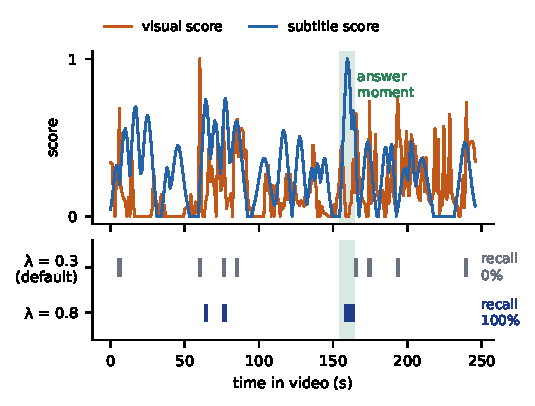
\includegraphics[width=\linewidth]{f01_teaser.pdf}\\
      {\scriptsize Real example: $\lam=0.3$ \bad{misses} the answer moment (green), $\lam=0.8$ \good{hits} it.}
    \end{column}
  \end{columns}
\end{frame}}

\newcommand{\titleframe}{%
{\setbeamertemplate{footline}{}\setbeamertemplate{frametitle}{}
\begin{frame}[t]\titlepage\end{frame}}}

\newcommand{\thankframe}{%
{\setbeamertemplate{footline}{}\setbeamertemplate{frametitle}{}
\begin{frame}[t]\mbzuaiThankYou\end{frame}}}
.
\usepackage{amsmath,amssymb}
\usepackage{booktabs}
\usepackage{xcolor}
\usetheme{MBZUAI}
\graphicspath{{assets/}{../figs/}}
\setbeamertemplate{navigation symbols}{}

\newcommand{\lam}{\lambda}
\newcommand{\strong}[1]{\textcolor{mbzuai-navy}{\textbf{#1}}}
\newcommand{\good}[1]{\textcolor{green!45!black}{\textbf{#1}}}
\newcommand{\bad}[1]{\textcolor{red!65!black}{\textbf{#1}}}

% ── Team and roles: edit here, all three decks update ─────────────────────
\newcommand{\roleJH}{Problem and setup; score cache and data pipeline; Q1 analysis; overall study (Q1--Q4)}
\newcommand{\roleLJ}{Continual learning experiments and analysis (Q2--Q3)}
\newcommand{\roleMA}{Downstream question-answering evaluation (Q4)}

\title[Fusion Weight for Keyframe Search]{Should the Fusion Weight Change with the Question?}
\institute[MBZUAI]{CV805 Course Project \\ Mohamed bin Zayed University of Artificial Intelligence}
\date{\today}
\titlelogos{assets/logo_dark.pdf}
\footleft{Should the Fusion Weight Change with the Question?}
\footright{\insertframenumber{} / \inserttotalframenumber}

% Team slide; #1 = JH, LJ or MA, the presenter's row is highlighted.
\usepackage{etoolbox}
\newcommand{\teamrow}[4]{% #1 key, #2 presenter key, #3 name, #4 role
  \ifstrequal{#1}{#2}%
    {\textbf{\textcolor{mbzuai-navy}{#3}} & \textbf{\textcolor{mbzuai-navy}{#4}} & \textcolor{mbzuai-dark-sand}{\textbf{this talk}}}%
    {\textcolor{mbzuai-subtle}{#3} & \textcolor{mbzuai-subtle}{#4} & }}
\newcommand{\teamframe}[1]{%
\begin{frame}{Team and my part}
  \centering
  \renewcommand{\arraystretch}{1.6}
  \begin{tabular}{p{0.27\textwidth}p{0.52\textwidth}p{0.11\textwidth}}
    \toprule
    Member & Main contribution & \\
    \midrule
    \teamrow{JH}{#1}{Jianxiang He}{\roleJH} \\
    \teamrow{LJ}{#1}{Longtao Jiang}{\roleLJ} \\
    \teamrow{MA}{#1}{Makhmud Assentay}{\roleMA} \\
    \bottomrule
  \end{tabular}
\end{frame}}

% Context frame used by every talk: VSI, the weight, and the example.
\newcommand{\contextframe}{%
\begin{frame}{Background: two clues, one weight}
  \begin{columns}[c,onlytextwidth]
    \begin{column}{0.47\textwidth}
      \small
      A VLM can only look at \strong{about 8 frames} of a long video, so we must pick them well.\\[2mm]
      VSI scores every second with two clues:
      \begin{itemize}
        \item \strong{Visual}: do the question's objects appear?
        \item \strong{Subtitle}: does the subtitle match the question?
      \end{itemize}
      \[ S(t) = (1-\lam)\,\text{visual}(t) + \lam\,\text{subtitle}(t) \]
      and keeps the top 8 seconds. VSI uses \strong{$\lam=0.3$ for every question}.
    \end{column}
    \begin{column}{0.5\textwidth}
      \centering
      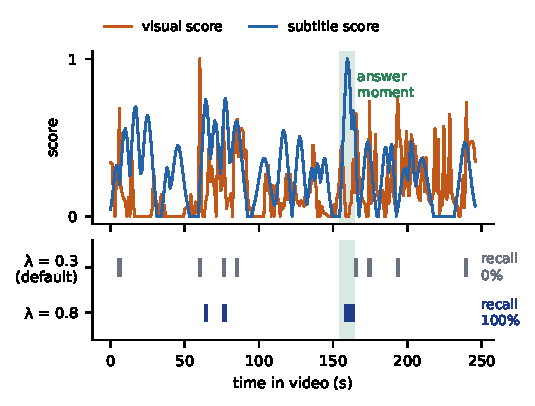
\includegraphics[width=\linewidth]{f01_teaser.pdf}\\
      {\scriptsize Real example: $\lam=0.3$ \bad{misses} the answer moment (green), $\lam=0.8$ \good{hits} it.}
    \end{column}
  \end{columns}
\end{frame}}

\newcommand{\titleframe}{%
{\setbeamertemplate{footline}{}\setbeamertemplate{frametitle}{}
\begin{frame}[t]\titlepage\end{frame}}}

\newcommand{\thankframe}{%
{\setbeamertemplate{footline}{}\setbeamertemplate{frametitle}{}
\begin{frame}[t]\mbzuaiThankYou\end{frame}}}

\subtitle{The Whole Study: Q1--Q4}
\author[Jianxiang He]{Jianxiang He \\ \small with Longtao Jiang and Makhmud Assentay}
\footmid{Jianxiang He}

\begin{document}
\titleframe
\teamframe{JH}
\contextframe

\begin{frame}{Our questions and my part}
  \begin{columns}[T,onlytextwidth]
    \begin{column}{0.5\textwidth}
      \begin{block}{Four research questions}
        \begin{enumerate}
          \item[Q1] Does the best $\lam$ depend on the question type?
          \item[Q2] Can a predictor learn $\lam$ as question types arrive one by one (continual learning)? Does it forget?
          \item[Q3] If the gain is small, why?
          \item[Q4] Do better frames give better answers?
        \end{enumerate}
      \end{block}
    \end{column}
    \begin{column}{0.46\textwidth}
      \strong{My part}
      \begin{itemize}
        \item Set up the problem and the benchmark: 753 LongVideoBench questions, 4 question types, 3 orders $\times$ 3 seeds
        \item Built the score cache and data pipeline
        \item Q1 analysis, and tied Q1--Q4 into one study
      \end{itemize}
      \vspace{1mm}
      {\small Longtao led Q2--Q3, Makhmud led Q4.}
    \end{column}
  \end{columns}
\end{frame}

\begin{frame}{Q1: types want different weights}
  \begin{columns}[c,onlytextwidth]
    \begin{column}{0.6\textwidth}
      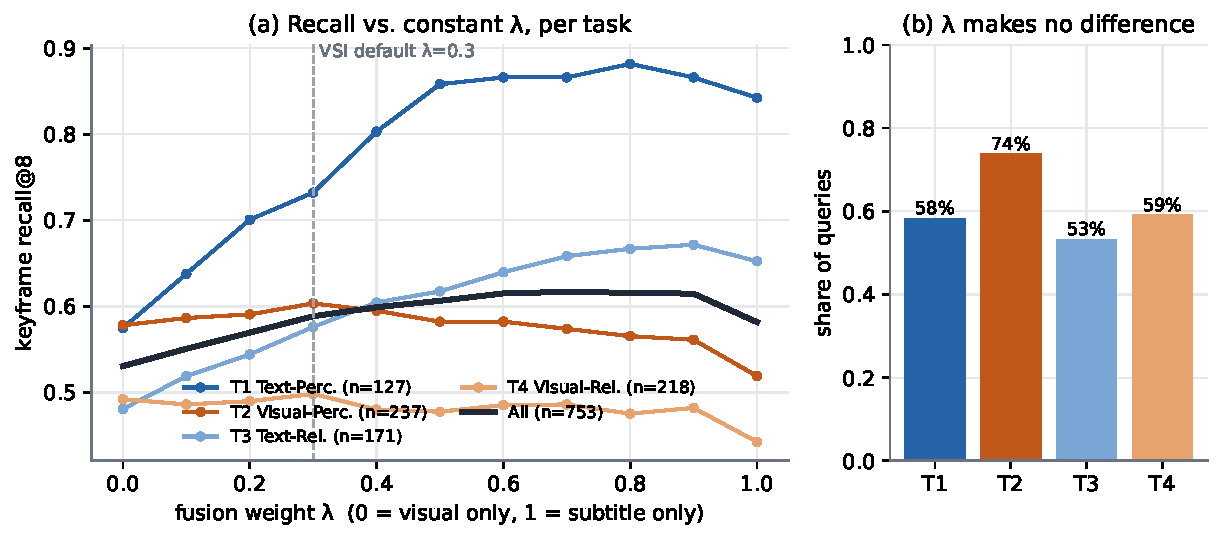
\includegraphics[width=\linewidth]{f02_headroom.pdf}
    \end{column}
    \begin{column}{0.37\textwidth}
      \small
      \begin{itemize}
        \item Text types best at $\lam=0.8$--$0.9$; visual types at $\le0.3$
        \item Per question: text \strong{0.62} vs.\ visual \strong{0.49}, $p=1.6\times10^{-6}$
        \item But \bad{53--74\%} of questions do not react to $\lam$
      \end{itemize}
    \end{column}
  \end{columns}
\end{frame}

\begin{frame}{Q1: where is the room to improve?}
  \begin{columns}[c,onlytextwidth]
    \begin{column}{0.58\textwidth}
      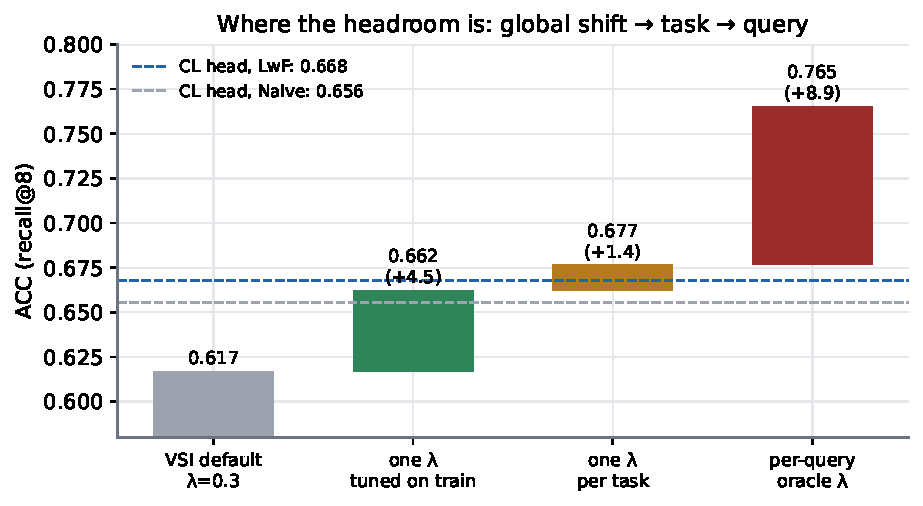
\includegraphics[width=\linewidth]{f16_decomp.pdf}
    \end{column}
    \begin{column}{0.39\textwidth}
      \begin{itemize}
        \item Tune one global $\lam$: \good{+4.5}
        \item One $\lam$ per type: \strong{+1.4} more
        \item Best $\lam$ per question: \strong{+8.9} more
      \end{itemize}
      \vspace{2mm}
      \begin{alertblock}{Q1 answer}
        Yes, the type matters; but most of the room is in \textbf{per-question} differences.
      \end{alertblock}
    \end{column}
  \end{columns}
\end{frame}

\begin{frame}{Q2--Q3: ties a tuned constant}
  \begin{columns}[c,onlytextwidth]
    \begin{column}{0.56\textwidth}
      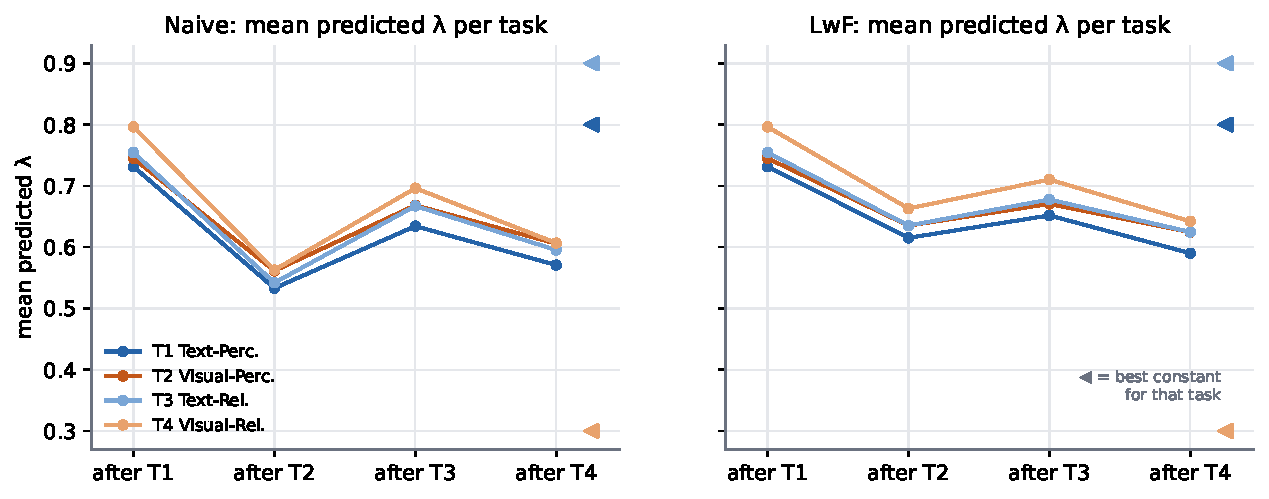
\includegraphics[width=\linewidth]{f12_lambda_rounds.pdf}
      {\scriptsize Predicted $\lam$ per type after each stage; triangles = best $\lam$ per type.}
    \end{column}
    \begin{column}{0.41\textwidth}
      \small
      \begin{itemize}
        \item Beats default $\lam=0.3$ by \good{4--5 points} in 9/9 runs
        \item vs.\ one \strong{tuned} $\lam$: only \bad{+0.6} (best method)
        \item Reason: it gives \strong{every type almost the same $\lam$} ($\approx$0.6)
        \item Forgetting is small; LwF halves it, but only in 6/9 runs
      \end{itemize}
    \end{column}
  \end{columns}
\end{frame}

\begin{frame}{Q4: helps only some questions}
  \begin{columns}[c,onlytextwidth]
    \begin{column}{0.6\textwidth}
      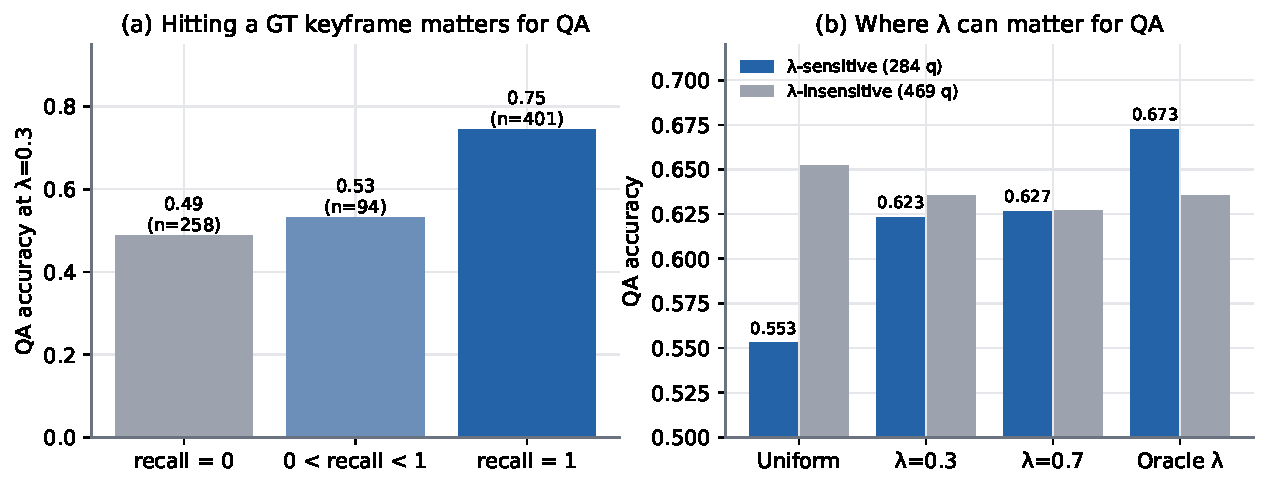
\includegraphics[width=\linewidth]{f15_qa_recall.pdf}
    \end{column}
    \begin{column}{0.37\textwidth}
      \small
      \begin{itemize}
        \item Qwen3-VL-8B: learned $\lam$ = default ($+0.4$, n.s.)
        \item Hitting the answer moment matters: \strong{0.49} vs.\ \strong{0.75}
        \item On the 284 questions where $\lam$ changes the frames, the best $\lam$ adds \good{5 points}
      \end{itemize}
    \end{column}
  \end{columns}
\end{frame}

\begin{frame}{Summary}
  \begin{enumerate}
    \item \strong{The best weight depends on the question type}, but most of the gain is per question.
    \vspace{2mm}
    \item \strong{Continual learning beats the default but only ties a tuned constant}; it collapses to one weight for all types.
    \vspace{2mm}
    \item \strong{Better frames help answers only where the weight changes the frames} (about 38\% of questions).
    \vspace{2mm}
    \item \strong{Lesson:} always compare a learned weight with a \emph{tuned} constant. Four silent bugs each reversed our conclusions along the way.
  \end{enumerate}
\end{frame}

\thankframe

% ════════════════════════════ backup for Q&A ════════════════════════════
\appendix

\begin{frame}{Backup: setup}
  \small
  \begin{columns}[T,onlytextwidth]
    \begin{column}{0.48\textwidth}
      \strong{Data}: LongVideoBench val, one question per video, 753 questions\\[1mm]
      \strong{Types}: T1 text perception (127), T2 visual perception (237), T3 text relation (171), T4 visual relation (218)\\[1mm]
      70/30 train/test split; orders T1-T2-T3-T4, T1-T3-T2-T4, T3-T1-T2-T4; 3 seeds\\[1mm]
      \strong{Predictor}: 2-layer MLP, 54 inputs from the two score curves, outputs a weighted average over 11 values of $\lam$
    \end{column}
    \begin{column}{0.48\textwidth}
      \strong{Methods}: Naive, EWC, LwF, ER, kNN, Joint (reference)\\[1mm]
      \strong{Baselines}: default 0.3; one $\lam$ tuned on train; one $\lam$ per type; per-question oracle\\[1mm]
      \strong{Metrics}: recall@8 (answer moments hit within $\pm$5 s); ACC = final average; FM = forgetting
    \end{column}
  \end{columns}
\end{frame}

\begin{frame}{Backup: main results (9 runs)}
  \centering\small
  \begin{tabular}{lcccc}
    \toprule
    Method & ACC $\uparrow$ & FM $\downarrow$ & vs.\ 0.3 & vs.\ tuned \\
    \midrule
    Default $\lam=0.3$ & 0.617 & -- & -- & $-$4.5 \\
    One tuned $\lam$ & 0.662 & -- & +4.5 & -- \\
    One $\lam$ per type & 0.677 & -- & +6.0 & +1.4 \\
    Oracle & 0.765 & -- & +14.8 & +10.3 \\
    \midrule
    Naive & 0.656 & 0.029 & +3.9 & $-$0.7 (3/9) \\
    EWC & 0.662 & 0.023 & +4.5 & $-$0.1 (4/9) \\
    LwF & 0.668 & 0.015 & +5.1 & +0.6 (7/9) \\
    ER & 0.660 & 0.021 & +4.3 & $-$0.3 (4/9) \\
    Joint (ref.) & 0.668 & 0.015 & +5.2 & +0.6 (6/9) \\
    kNN & 0.645 & 0.005 & +2.9 & $-$1.7 (0/9) \\
    \bottomrule
  \end{tabular}
\end{frame}

\begin{frame}{Backup: four silent bugs}
  \small
  \begin{tabular}{p{0.24\textwidth}p{0.68\textwidth}}
    \toprule
    Problem & What happened \\
    \midrule
    Frames vs.\ seconds & Annotations in frames, scores per second: 94\% of questions got zero recall. \\
    Annotation frame rate & LongVideoBench counts frames at a fixed \strong{24 fps}, not the real 30 fps (38/39 vs.\ 14/39 match the answer subtitle). \\
    Short videos dropped & Videos $\le$16 s could not fill VSI's 4$\times$4 grid and were silently skipped (197 questions). \\
    Train vs.\ test weight & Trained on the average $\lam$, tested on the most likely one ($\lam=0$ or $1$): learned weights looked 3--5 points \bad{worse} than the default. \\
    \bottomrule
  \end{tabular}
\end{frame}

\begin{frame}{Backup: text vs.\ visual}
  \centering
  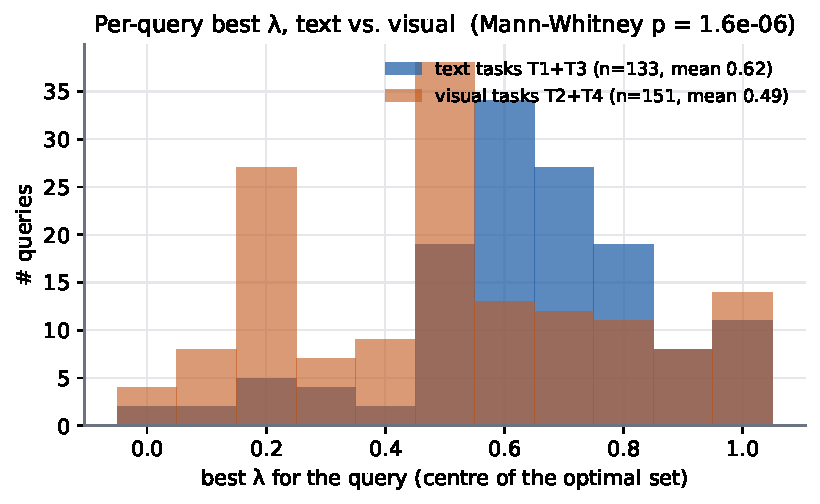
\includegraphics[height=0.72\textheight]{f03_premise.pdf}
\end{frame}

\begin{frame}{Backup: run by run}
  \centering
  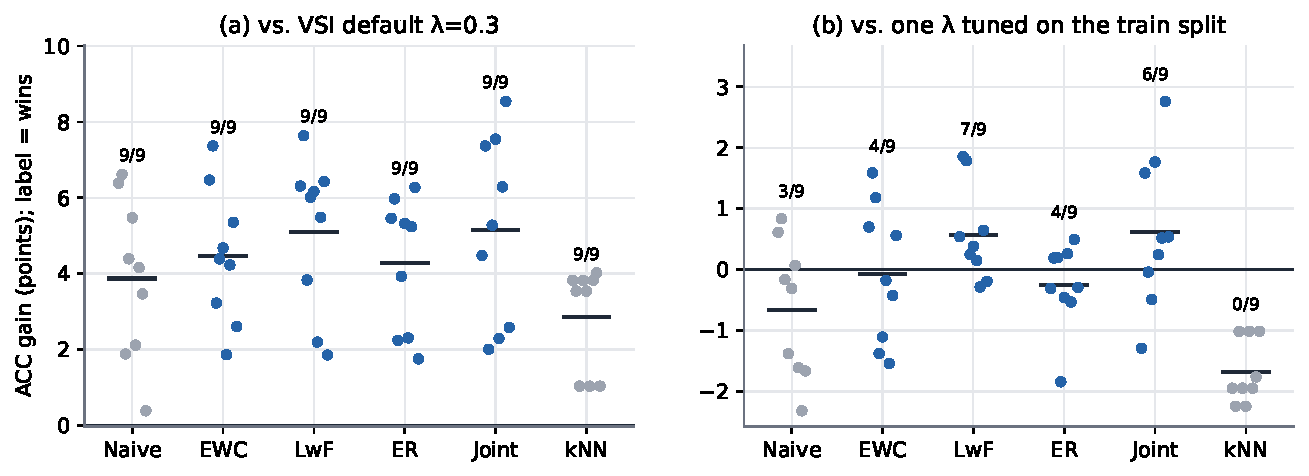
\includegraphics[width=0.9\textwidth]{f10_paired.pdf}
\end{frame}

\end{document}
